\documentclass[12pt, a4papre]{article}
\usepackage[catalan]{babel}
\usepackage[unicode]{hyperref}
\usepackage{amsmath}
\usepackage{amssymb}
\usepackage{amsthm}
\usepackage{xifthen}
\usepackage{siunitx}
\usepackage{xcolor}
\usepackage{float}
\usepackage{listings}
\usepackage{setspace}
\usepackage{graphicx}
\usepackage{tikz,lipsum,lmodern}
\usepackage[most]{tcolorbox}
\usepackage{circuitikz}
\usepackage{indentfirst}
\usepackage{verbatimbox}
\usepackage[T1]{fontenc}
\usepackage{beramono}% monospaced font with bold variant
 \usepackage{tikz-timing}[2009/05/15]
\usepackage{listings}
\lstdefinelanguage{VHDL}{
   morekeywords={
     library,use,all,entity,is,port,in,out,end,architecture,of,
     begin,and
   },
   morecomment=[l]--
}
 
\usepackage{xcolor}
\colorlet{keyword}{blue!100!black!80}
\colorlet{comment}{green!50!black!90}
\lstdefinestyle{vhdl}{
   language     = VHDL,
   basicstyle   = \ttfamily,
   keywordstyle = \color{keyword}\bfseries,
   commentstyle = \color{comment}
}

\graphicspath{ {./Imatges/} }


\newcommand{\norm}[1]{\lvert #1 \rvert}

\hypersetup{
    colorlinks = true,
    linkcolor = blue
}

\author{Daniel Vilardell\\
	   Igor Yuziv}
\title{Previ DGD practica 2}
\date{}

\begin{document}
	\maketitle

	\textcolor{blue}{Pregunta 1:} \textbf{Per dissenyar el bloc combinacional AxB aprofiteu part del disseny fet en la pràctica anterior, on justament es feia un multiplicador. Expliqueu com era aquest disseny i quines modificacions cal fer-li per poder utilitzar-lo a ppal.}\\\\
	
	Per tal de fer el bloc AxB, usarem el bloc multiplicador realitzat a la practica anterior, el que com que l'entrada es de dos nombres de 4 bits mentres que el component multiplicador se li entren dos entrades de 8 bits, haurem de fer un conversor de nombres en binari de 4 a 8 bits. La sortida ens la donara en binari, per a passarla a BCD usarem un component programat amb vhdl que considerarà tots els possibles nombres solucio i assignarà al resultat el que li toqui.
	
	Primer de tot farem un breu resum de com funcionava el multiplicador. Aquest feia la multiplicació escolar, es a dir, colocava un nombre a dalt i un a baix i multiplicava xifra per xifra. A mesura que anava multiplicant extreia el nombre de menys pes de cada producte individual i el situava a la sortida. Els altres digits els sumava amb el seguent. Això fins als ultims digits que tots eren destinats al output.
	
	El component conversor de 4 a 8 bits serà el seguent
	
	\begin{figure}[H]
		\begin{center}
		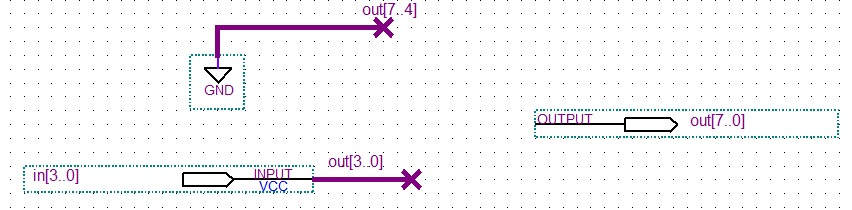
\includegraphics[width=150mm]{Pregunta1_1.jpeg}
		\end{center}
	\end{figure}
	
	El component que ens convertira la sortida del multiplicador de binari a BCD es el següent.
	\begin{lstlisting}[style=vhdl, frame=single, basicstyle=\tiny]
LIBRARY ieee; USE ieee.std_logic_1164.ALL;  

ENTITY BIN_BCD_8B IS PORT (   
	BIN : IN STD_LOGIC_VECTOR(7 downto 0);   
	BCD : OUT STD_LOGIC_VECTOR(7 downto 0)); 
END BIN_BCD_8B;  

ARCHITECTURE taula_veritat OF BIN_BCD_8B IS   
	BEGIN 
	with BIN SELECT BCD <=     	
		"10011001" WHEN "00111000",  -- 81     
		"01110010" WHEN "01001000",  -- 72      
		"01100100" WHEN "01000000",  -- 64     
		"01010110" WHEN "00111000",  -- 56     
		"01010100" WHEN "00111000",  -- 54     
		"00101000" WHEN "00011100",  -- 28     
		"01001001" WHEN "00110001",  -- 49     
		"01001000" WHEN "00110000",  -- 48     
		"01000101" WHEN "00101101",  -- 45     
		"01000010" WHEN "00101010",  -- 42     
		"01000000" WHEN "00101000",  -- 40     
		"00110110" WHEN "00100100",  -- 36     
		"00110101" WHEN "00100011",  -- 35     
		"00110010" WHEN "00100000",  -- 32     
		"00110000" WHEN "00011110",  -- 30     
		"00101000" WHEN "00011100",  -- 28     
		"00100110" WHEN "00011011",  -- 27     
		"00100101" WHEN "00011001",  -- 25     
		"00100100" WHEN "00011000",  -- 24     
		"00100001" WHEN "00010101",  -- 21     
		"00100000" WHEN "00010100",  -- 20     
		"00011000" WHEN "00010010",  -- 18     
		"00010110" WHEN "00010000",  -- 16     
		"00010101" WHEN "00001111",  -- 15     
		"00010100" WHEN "00001110",  -- 14     
		"00010010" WHEN "00001100",  -- 12     
		"00010000" WHEN "00001010",  -- 10     
		"00001001" WHEN "00001001",  -- 9     
		"00001000" WHEN "00001000",  -- 8     
		"00000111" WHEN "00000111",  -- 7     
		"00000110" WHEN "00000110",  -- 6     
		"00000101" WHEN "00000101",  -- 5     
		"00000100" WHEN "00000100",  -- 4    
		"00000011" WHEN "00000011",  -- 3     
		"00000010" WHEN "00000010",  -- 2     
		"00000001" WHEN "00000001",  -- 1     
		"00000000" WHEN "00000000",  -- 0     
		"--------" WHEN OTHERS;   
END taula_veritat;
\end{lstlisting}

	\textcolor{blue}{Pregunta 2:} \textbf{Dissenyeu el mòdul combinacional sel en forma de logigrama amb un nombre mínim de portes lògiques estàndard.} 
	 
	Per a fer la seleccio usarem un multiplexor 2:1 per a busos de 8 bits. Aquest estarà composat per 8 multiplixors 2:1 classics de un bit de la forma
	\begin{figure}[H]
		\begin{center}
		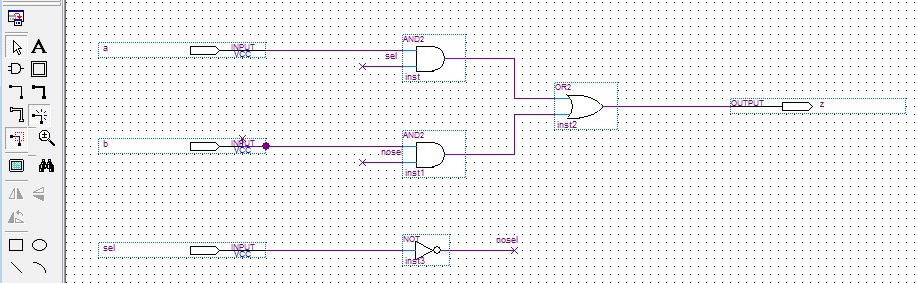
\includegraphics[width=130mm]{multiplexor2_1.jpeg}
		\end{center}
	\end{figure}
	
	Per tant a una de les entrades de informació se li posara AxB i a l'altre un vector "1111111", ja que si el bit es 1 el segment de la placa esta apagat. I a la entrada de seleccio li posarem show.
	
	\textcolor{blue}{Pregunta 3:} \textbf{Dissenyeu el mòdul combinacional keygroup en forma de logigrama amb un nombre mínim de portes lògiques estàndard.}
	
	En primer lloc construirem una taula de veritat
	
	\begin{center}
	\begin{tabular}{||c| c c c c | c c c||} 
	 \hline
	 Tecla & $kc_3$ & $kc_2$ & $ kc_1 $ &$kc_0$ & BCD & AST & COI \\ [0.5ex] 
	 \hline\hline
	 0 & 0 & 0 & 0 & 0 & 1 & 0 & 0\\ 
	 \hline
	 1 & 0 & 0 & 0 & 1 & 1 & 0 & 0\\ 
	 \hline
	 2 & 0 & 0 & 1 & 0 & 1 & 0 & 0\\ 
	 \hline
	 3 & 0 & 0 & 1 & 1 & 1 & 0 & 0\\ 
	 \hline
	 4 & 0 & 1 & 0 & 0 & 1 & 0 & 0\\ 
	 \hline
	 5 & 0 & 1 & 0 & 1 & 1 & 0 & 0\\ 
	 \hline
	 6 & 0 & 1 & 1 & 0 & 1 & 0 & 0\\ 
	 \hline
	 7 & 0 & 1 & 1 & 1 & 1 & 0 & 0\\ 
	 \hline
	 8 & 1 & 0 & 0 & 0 & 1 & 0 & 0\\ 
	 \hline
	 9 & 1 & 0 & 0 & 1 & 1 & 0 & 0\\ 
	 \hline
	 A & 1 & 0 & 1 & 0 & 0 & 0 & 0\\ 
	 \hline
	 B & 1 & 0 & 1 & 1 & 0 & 0 & 0\\ 
	 \hline
	 C & 1 & 1 & 0 & 0 & 0 & 0 & 0\\ 
	 \hline
	 D & 1 & 1 & 0 & 1 & 0 & 0 & 0\\ 
	 \hline
	 * & 1 & 1 & 1 & 0 & 0 & 0 & 1\\ 
	 \hline
	 \# & 1 & 1 & 1 & 1 & 0 & 1 & 0\\ 
	  \hline\hline
	\end{tabular}
	\end{center}
	
	D'aqui podem veure rapidament les formules que tindran les funcions AST i COI
	\[AST = kc_3\cdot kc_2\cdot kc_1 \cdot \bar{kc_0}\]
	\[COI = kc_3\cdot kc_2\cdot kc_1 \cdot kc_0\]
	
	Per a la última sortida, la BCD construirem una taula de Karnaugh i agruparem uns per a trobar suma de minterms.
	
	\begin{center}
	\begin{tabular}{c|| c c c c} 
	 BCD & 00 & $01$ &$11$ & 10\\ [0.5ex] 
	 \hline\hline
	 00 & 1 & 1 & 1 & 1\\ 

	 01 & 1 & 1  & 1 & 1\\

	 11 & 0 & 0 & 0 & 0\\

	 10 & 1 & 1 & 0 & 0\\
	\end{tabular}
	\end{center}
	
	Veiem que podem fer un grup de 8 uns i un altre grup de quatre, per tant el resultat final es el següent
	\[BCD = \bar{kc_3} + \bar{kc_1}\cdot \bar{kc_4}\]
	
	Ara doncs ja podem construir el diseny amb el minim de portes and, or i not i tindrà la seguent forma
	\begin{figure}[H]
		\begin{center}
		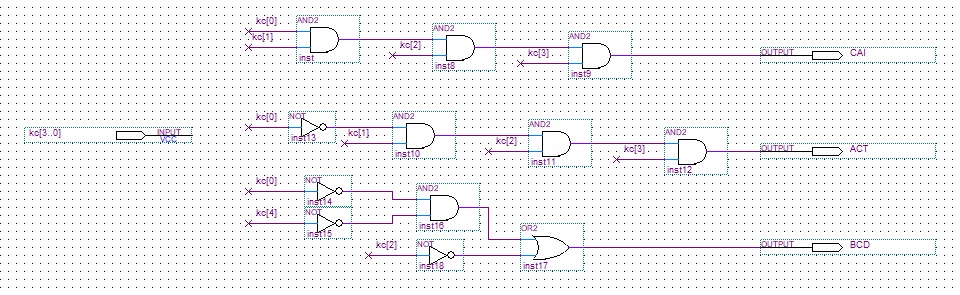
\includegraphics[width=130mm]{sel.jpeg}
		\end{center}
	\end{figure}
	
	\textcolor{blue}{Pregunta 4:} \textbf{Dissenyeu el mòdul combinacional leds en forma de logigrama amb un nombre mínim de portes lògiques estàndard. Aquest mòdul es descriu en l’apartat 3.2.}
	
	Aquest modul es ben senzill, nomes caldra rebre la entrada show, i a les sortides de leds vermells treure show, i a les de led verd show negat. Per tant tindra la seguent forma.
	\begin{figure}[H]
		\begin{center}
		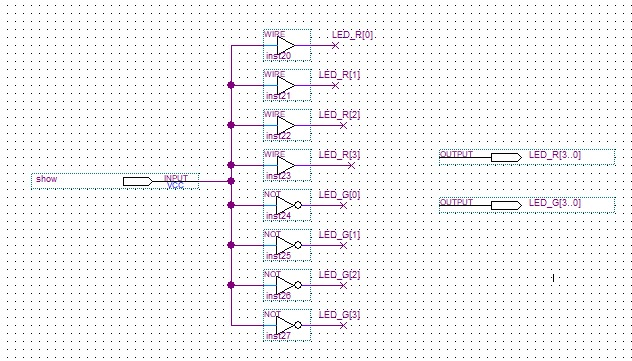
\includegraphics[width=110mm]{leds.jpeg}
		\end{center}
	\end{figure}
	
	\textcolor{blue}{Pregunta 5:}\textbf{Expliqueu	quina	és	la	 finalitat	i	com	 funciona	el	mòdul	regs.	Empleneu les	línies	 OpA[] i	OpB[] del	cronograma-exemple	donat	a	sota.}
	
	La finalitat del mòdul regs és guardar dos digits introduïts per teclat. El funcionament del mòdul és a partir de 2 registres de 4 bits agafà i guarda en la memòria el valor de l'entrada de manera que cada vegada que  \textbf{intro} està actiu, el valor prèviament guardat al primer registre passa al segon, canviant aquest primer el seu valor per l’introduït al teclat.
	També quan nrst = 0 els valors de OpA[] i OpB[] es posen a 0.	
		\begin{figure}[H]
		\begin{center}
		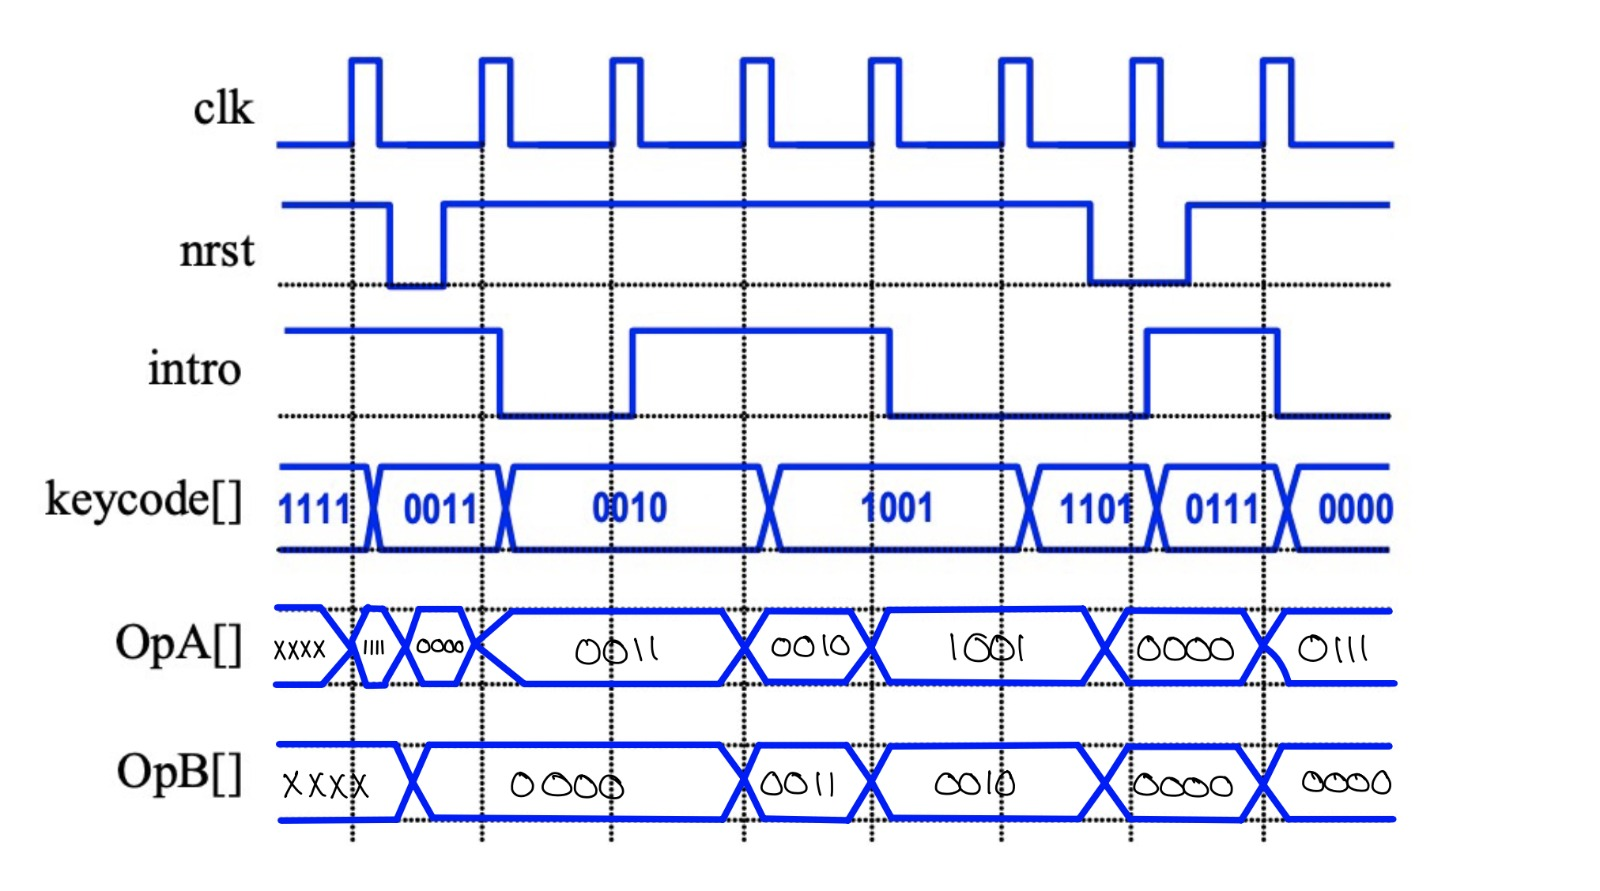
\includegraphics[width=110mm]{pregunta5.jpeg}
		\end{center}
	\end{figure}
	
	\textcolor{blue}{Pregunta 6:}\textbf{Dibuixeu	el	diagrama	d’estats	del	mòdul control.	Aquest	diagrama	ha	d’especificar	tan	els	canvis	d’estat	com	les	sortides.	}
	\begin{figure}[H]
		\begin{center}
		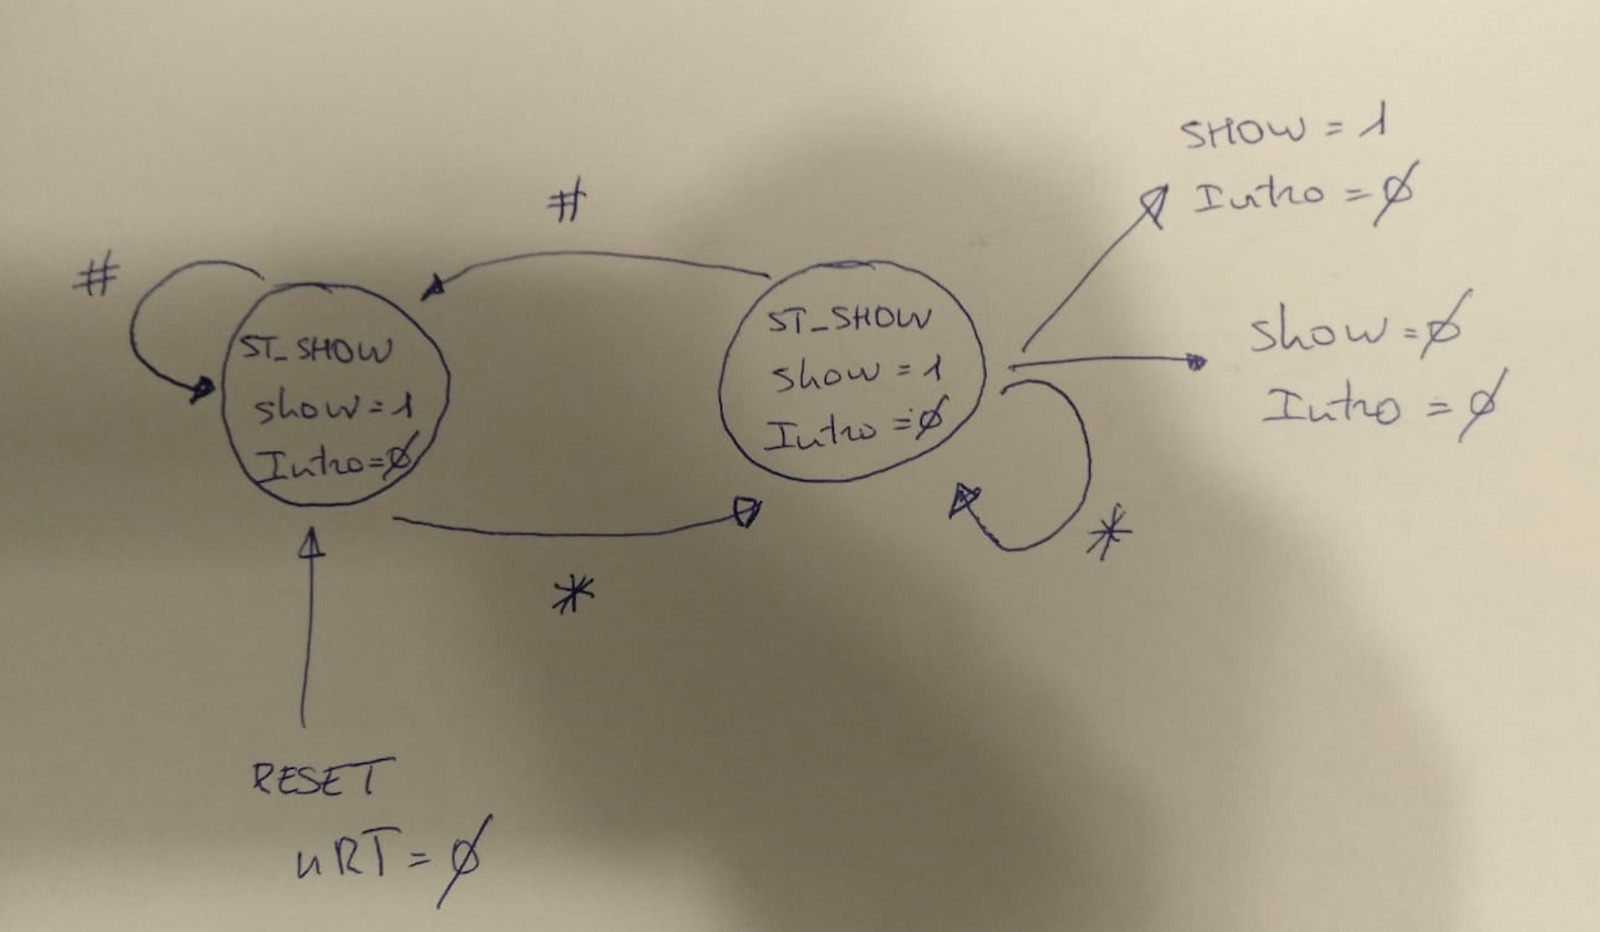
\includegraphics[width=110mm]{pregunta6.jpeg}
		\end{center}
	\end{figure}
	
	\textcolor{blue}{Pregunta 7:}\textbf{Expliqueu	el	funcionament	del	mòdul	control.	Empleneu	les	línies state,	show i	intro del	cronograma-exemple	donat	a	sota.	}
	
	El funcionament del mòdul control es gestionar el mòdul ppal per saber si te que mostrar la informació $(show)$ i introduïr $(intro)$ i també ast i coi ens indica quan estem introduïnt valors i quan volem que és mostrin i es calculin.
	Bcd ens indica si hem introduït una lletra o un valor.
	
	\begin{figure}[H]
		\begin{center}
		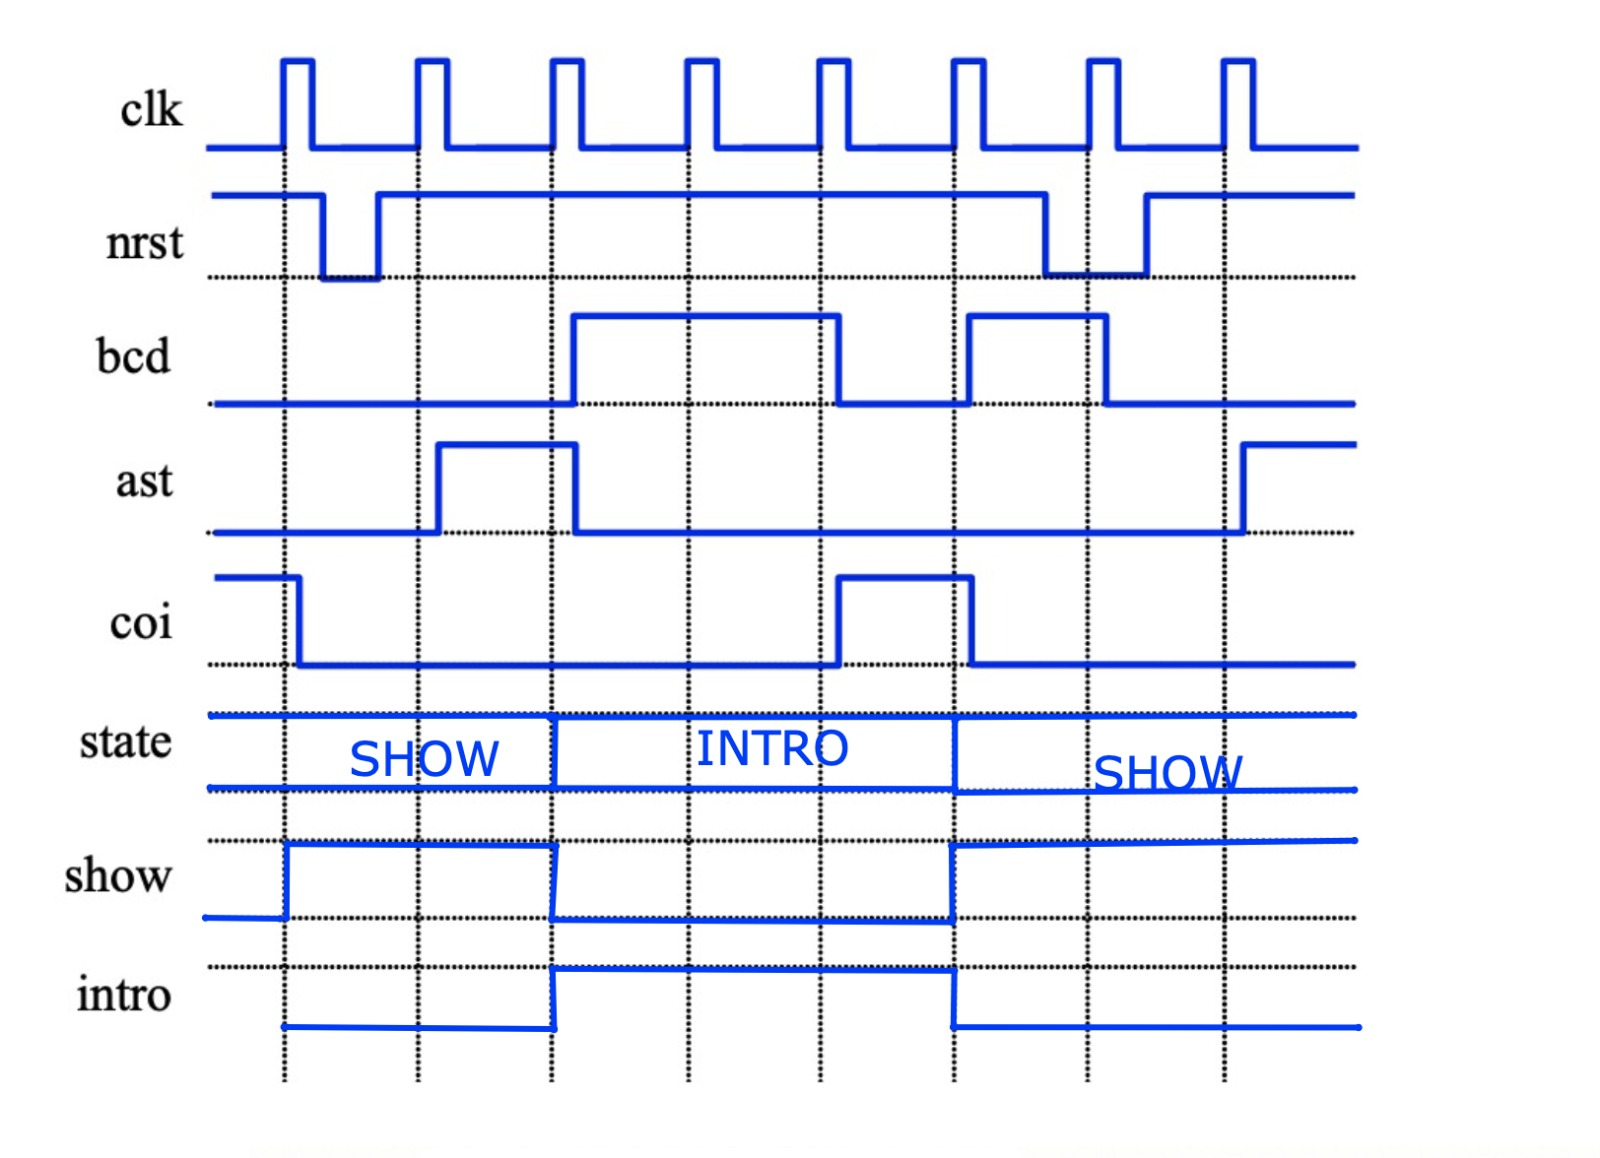
\includegraphics[width=110mm]{pregunta7.jpeg}
		\end{center}
	\end{figure}
	
	
	
\end{document}